%
% 電気関係学会九州支部連合会大会論文集用
% LaTeX テンプレート
%
% paper.tex, Ver. 1.12  June 16, 2004
% 作成者 苣木 禎史 (Yoshifumi CHISAKI)
%        高田 俊亨 (Toshimichi TAKADA)
%        田中 直哉 (Naoya TANAKA)
%        {chisaki@, toshimichi@hicc, naoya@hicc.}cs.kumamoto-u.ac.jp
%        熊本大学 工学部 情報システム工学科
%        ヒューマンインターフェース講座
%        サイバーコミュニケーション研究室
%
%        高橋 規一(Norikazu TAKASHI)
%        九州大学 大学院システム情報科学研究院 情報工学部門 

% 原稿を作成の際には,必ず原稿作成上の注意をお読みの上
% 作成ください。提出の際には,十分に推敲下さい。
%

% 1カラム
%\documentclass[a4j,10pt]{jceee-kyushu-euc}

% 2カラム
\documentclass[a4j,twocolumn,10pt]{jceee-kyushu-euc}

% 図を利用する場合
% \usepackage{graphicx}
% 文章を枠で囲む場合
\usepackage{ascmac}
% \usepackage{multirow}
% \usepackage{url}

\usepackage[dvipdfmx]{graphicx}
\usepackage{verbatim} % コメントアウトしてくれる便利なプリアンブルが使える \begin{comment} ... \end{comment}
\usepackage{txfonts}
\usepackage{setspace}
\usepackage{url}
% \usepackage[dvipdfmx]{hyperref}
% \usepackage{pxjahyper} %%hyperref読み込みの直後に
\usepackage{multirow}
\usepackage{enumitem}
\usepackage{makecell}

%\renewcommand{\baselinestretch}{0.85}% <- 行間を調整できます。
\newcommand{\diagramName}{SwiftDiagram}

%論文タイトル
%1行に収まるときは,2行目は必ず空行を入れてください。
\title{
      自然言語仕様とVDM++仕様の対応関係を自動で抽出する手法の提案\newline
}

\author{
高橋朋弘 片山徹郎\\
}

\affiliation{
宮崎大学大学院 工学研究科 工学専攻\\
}
%Emailはオプションです。書かない場合は,空行が出力されるように
%下記のようにチルダのままにしておいてください。
%書く場合は,チルダを削除してメールアドレスが1行出力されるように
%してください。
\emailaddress{
~
%\{author1, author2\}@jceee-kyushu.jp, author3@jceee-example.jp 
}
\begin{document}
\maketitle



\section{はじめに}
ソフトウェア開発における仕様策定段階では、自然言語による記述から始まることが一般的である。% 欲を言えばここで参考文献
しかし、自然言語には曖昧性が伴うため、プログラマが、仕様書の記述内容を、本来意図していない意味でとらえてしまうことや、
仕様書に明示されていない要件が存在し、本来満たすべき機能や制約が設計や実装の段階で考慮されないことといった問題が発生し得る\cite{spec_introduction}。

この問題を解決する手法の1つとして、形式手法がある\cite{successful_example}。
形式仕様を用いることで、自然言語の持つ曖昧性を排除し、厳密な仕様を作成することができる。
また、形式仕様記述言語の1つにVDM++(Vienna Development Method \cite{vdm})がある。% 参考文献

以上のことから、ソフトウェア開発における仕様策定段階では、自然言語と形式手法の両者を組み合わせた仕様策定が行われる場合がある。
しかし、自然言語と形式手法の併用には、仕様の変更や修正を行うたびに双方の記述を更新する必要があり、
その際に対応漏れが発生する可能性がある。
また、自然言語仕様と形式仕様のトレーサビリティを維持したまま、仕様を変更や修正する作業には手間と時間がかかる。

そこで、本論文では、自然言語仕様とVDM++仕様のトレーサビリティの維持を支援することを目的として、両仕様の対応関係を自動で抽出する手法を提案する。

\section{提案手法}
提案手法は、あらかじめ対応が取れている自然言語仕様とVDM++仕様に対して、自然言語処理を適用する。
そして、単語や構文の類似性に基づいて両仕様を比較し、対応関係を抽出する。

提案手法は、自然言語仕様の各要求仕様とVDM++仕様の各定義を1つの単位として、対応関係を抽出する。

\subsection{対象となる仕様書}
提案手法は、日本語で記述した自然言語仕様とVDM++仕様を対象とする。
また、対象となる自然言語仕様とVDM++仕様は事前に対応が取れていることを前提とする。

VDM++仕様の各定義について、対応関係を抽出する規則を、表\ref{tab:correspondence_rule}に示す。
提案手法は、対応関係のある自然言語仕様書の要求仕様とVDM++仕様書の定義が、表\ref{tab:correspondence_rule}の規則を満たす場合、
対応関係を抽出する。

% \begin{table}[t]
%     \centering
%     \caption{対応関係を抽出する規則}
%     \label{tab:correspondence_rule}
%     \begin{tabular}{c|l}
%         対象定義   & \multicolumn{1}{c}{規則}                        \\ \hline\hline
%         クラス定義 & \makecell[l]{識別子が、対応関係のある要求仕様内 \\の名詞である} \\ \hline
%         型定義     & \makecell[l]{識別子が、対応関係のある要求仕様内 \\の名詞の組み合わせである}               \\ \hline
%         定数値定義 & \makecell[l]{識別子が、対応関係のある要求仕様内 \\
%             の名詞の組み合わせであり、要求仕様                       \\
%             内で明記してある数値を定数値として                       \\
%             定義している}                                            \\ \hline
%         \makecell[c]{インスタンス                                    \\変数定義} & 型定義と同様       \\ \hline
%         操作定義   & \makecell[l]{識別子が、対応関係のある要求仕様内 \\
%             と同様な目的語と述語の係り受け関係                       \\
%             を持っている}                                            \\ \hline
%         関数定義   & 操作定義と同様                                  \\ \hline
%     \end{tabular}
% \end{table}

\begin{table}[t]
      \centering
      \caption{対応関係を抽出する規則}
      \label{tab:correspondence_rule}
      \normalsize
      \begin{tabular}{c|l}
            対象定義   & \multicolumn{1}{c}{規則}                         \\ \hline\hline
            クラス定義 & \makecell[l]{識別子が要求仕様内の名詞と一致する} \\ \hline
            型定義     & \makecell[l]{識別子内の複数名詞が要求仕様の名詞  \\群にすべて含まれる}           \\ \hline
            定数値定義 & \makecell[l]{型定義と同様                        \\値の一致にも注目する}                           \\ \hline
            \makecell[c]{インスタンス                                     \\変数定義} & 型定義と同様       \\ \hline
            操作定義   & \makecell[l]{識別子内の述語と目的語の係り受け関  \\係が、要求仕様内にも存在する} \\ \hline
            関数定義   & 操作定義と同様                                   \\ \hline
      \end{tabular}
\end{table}

\subsection{対応関係の抽出}
提案手法では、自然言語仕様とVDM++仕様の対応関係を自動的に抽出するために、以下の手順に従って処理を行う。

\begin{enumerate}
      \setlength{\itemsep}{-2pt}
      \item 要求仕様の名詞抽出\\
            まず、自然言語仕様書の要求仕様を形態素解析し、名詞を抽出する。
            抽出した名詞は、後続の処理において識別子との照合対象となる。
      \item クラス定義との対応\\
            VDM++仕様内のクラス定義の識別子が、要求仕様から抽出した名詞と一致する場合、
            その要求仕様とクラス定義との間に対応関係を設定する。
      \item 型定義およびインスタンス変数定義との対応\\
            VDM++仕様内の型定義またはインスタンス変数定義の識別子内のすべての名詞が、
            要求仕様から抽出した名詞と一致する場合、その要求仕様との間に対応関係を設定する。
      \item 定数値定義との対応\\
            定数値定義については、3.の処理に加え、定数値定義の値を、要求仕様が含んでいた場合、対応関係を設定する。
      \item 操作定義および関数定義との対応\\
            操作定義または関数定義の識別子に対して構文解析を行い、述語と目的語の係り受け関係を抽出する。
            さらに、要求仕様において同様の係り受け関係を持つ記述を特定し、その構造的一致に基づいて対応関係を設定する。
\end{enumerate}

対応関係のある自然言語仕様とVDM++仕様を、図\ref{fig:sample_text}に示す。

\begin{figure}[tp]
      \centering
      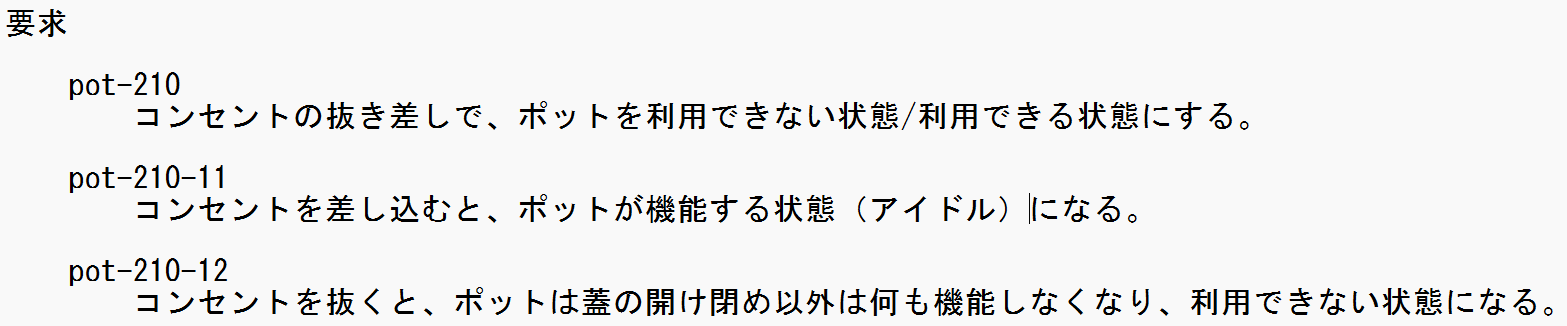
\includegraphics[width=\columnwidth]{../image/jceee/sample_text2.png}
      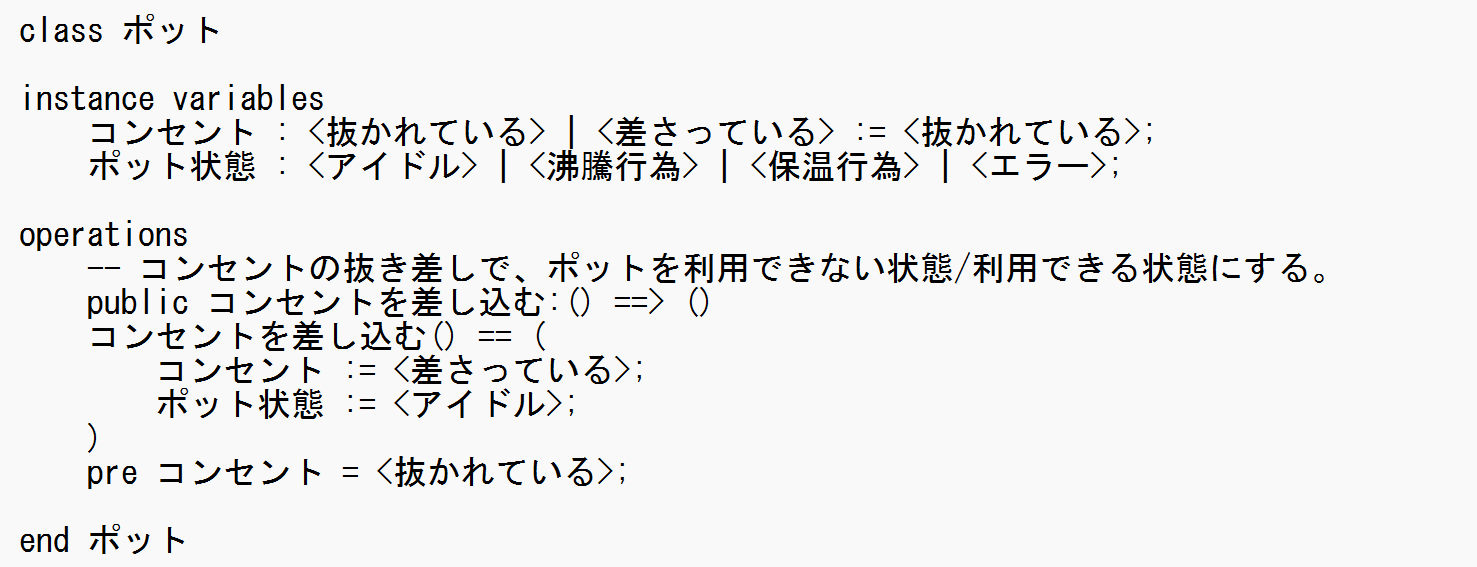
\includegraphics[width=\columnwidth]{../image/jceee/vdm_example.png}
      \caption{対応関係のある自然言語仕様書(上)およびVDM++仕様書(下)}
      \label{fig:sample_text}
\end{figure}

図\ref{fig:sample_text}に示す、クラス定義「ポット」は、識別子が「ポット」である。
要求仕様「pot-210」、「pot-210-11」、「pot-210-12」は、名詞「ポット」を含んでいるため、
クラス定義「ポット」と要求仕様「pot-210」、「pot-210-11」、「pot-210-12」の対応関係を抽出する。

インスタンス変数定義「ポット状態」の識別子「ポット状態」は、「ポット」と「状態」の 2 つの名詞からなる。
要求仕様「pot-210」と「pot-210-11」は、名詞「ポット」と「状態」のどちらも含んでいるため、
インスタンス変数定義「ポット状態」と要求仕様「pot-210」、「pot-210-11」の対応関係を抽出する。

操作定義「コンセントを差し込む」の識別子「コンセントを差し込む」は、
目的語である文節「コンセントを」が述語である文節「差し込む」に係っている。
要求仕様「pot-210-11」がこれと同様な係り受け関係を含んでいるため、操作定義「コンセントを差し込む」と要求仕様「pot-210-11」の対応関係を抽出する。

\section{適用例}
提案手法の適用対象として、IPA独立行政法人情報処理推進機構が公開している資料「厳密な仕様記述入門」\cite{spec_introduction}で例題として用いられている、
エレベータを対象とする自然言語仕様とVDM++仕様を参考に、表\ref{tab:correspondence_rule}の規則を満たす状態の、
自然言語仕様とVDM++仕様を作成した。
作成した自然言語仕様の一部を、図\ref{fig:nat_elevater}に、VDM++仕様の一部を、図\ref{fig:vdm_elevater}に示す。

\begin{figure}[tp]
      \centering
      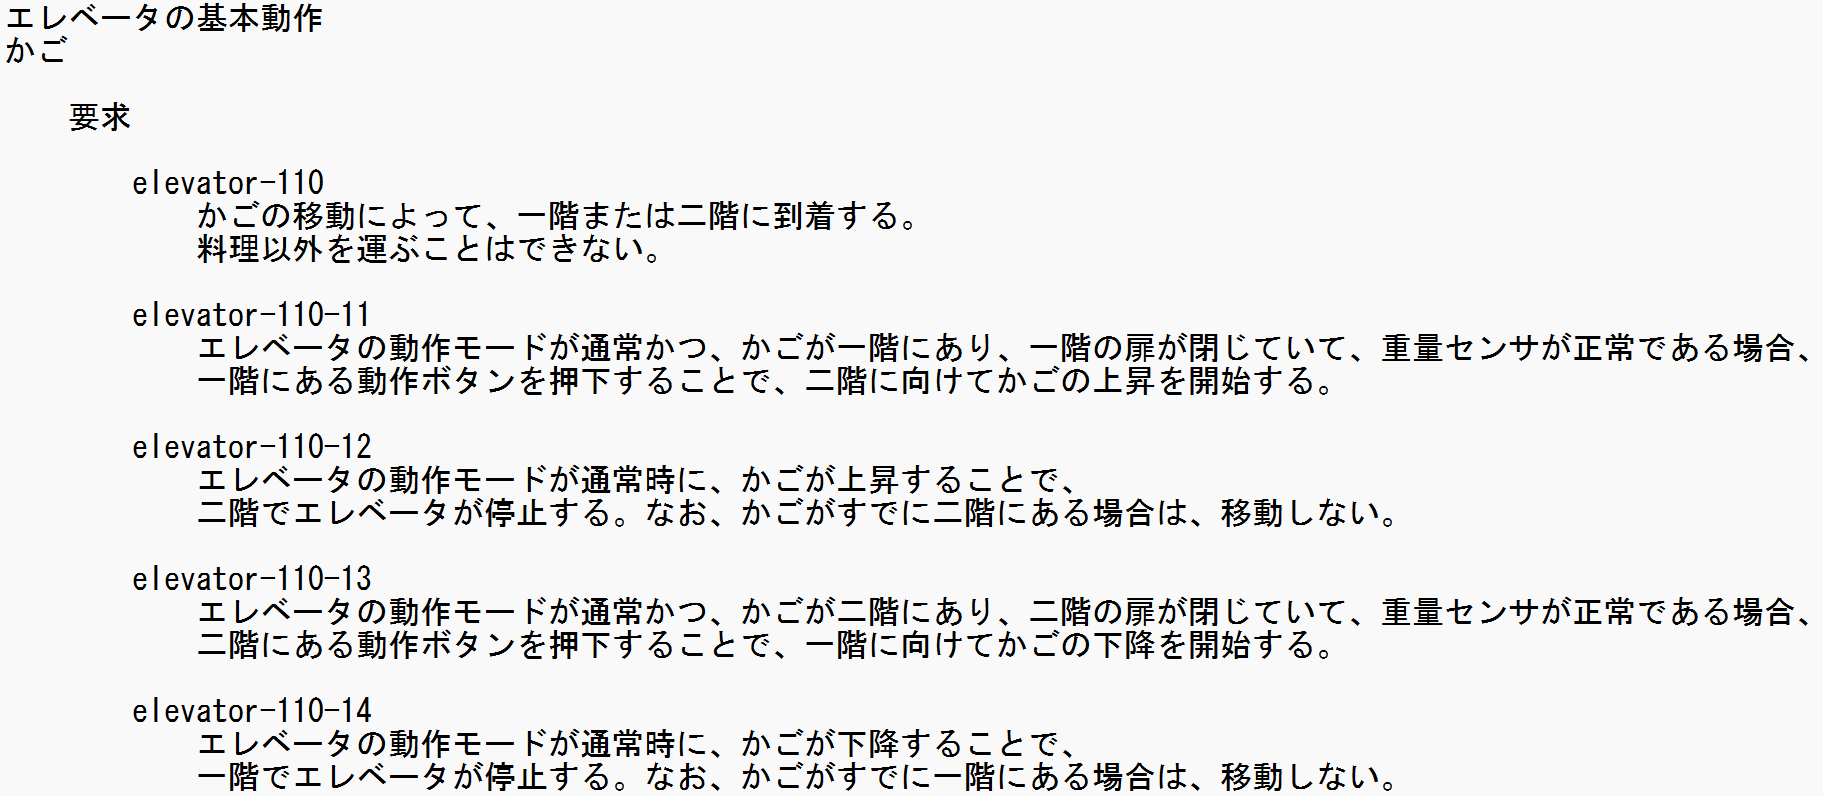
\includegraphics[width=\columnwidth]{../image/jceee/elevater.png}
      \caption{作成した自然言語仕様の一部}
      \label{fig:nat_elevater}
\end{figure}

\begin{figure}[tp]
      \centering
      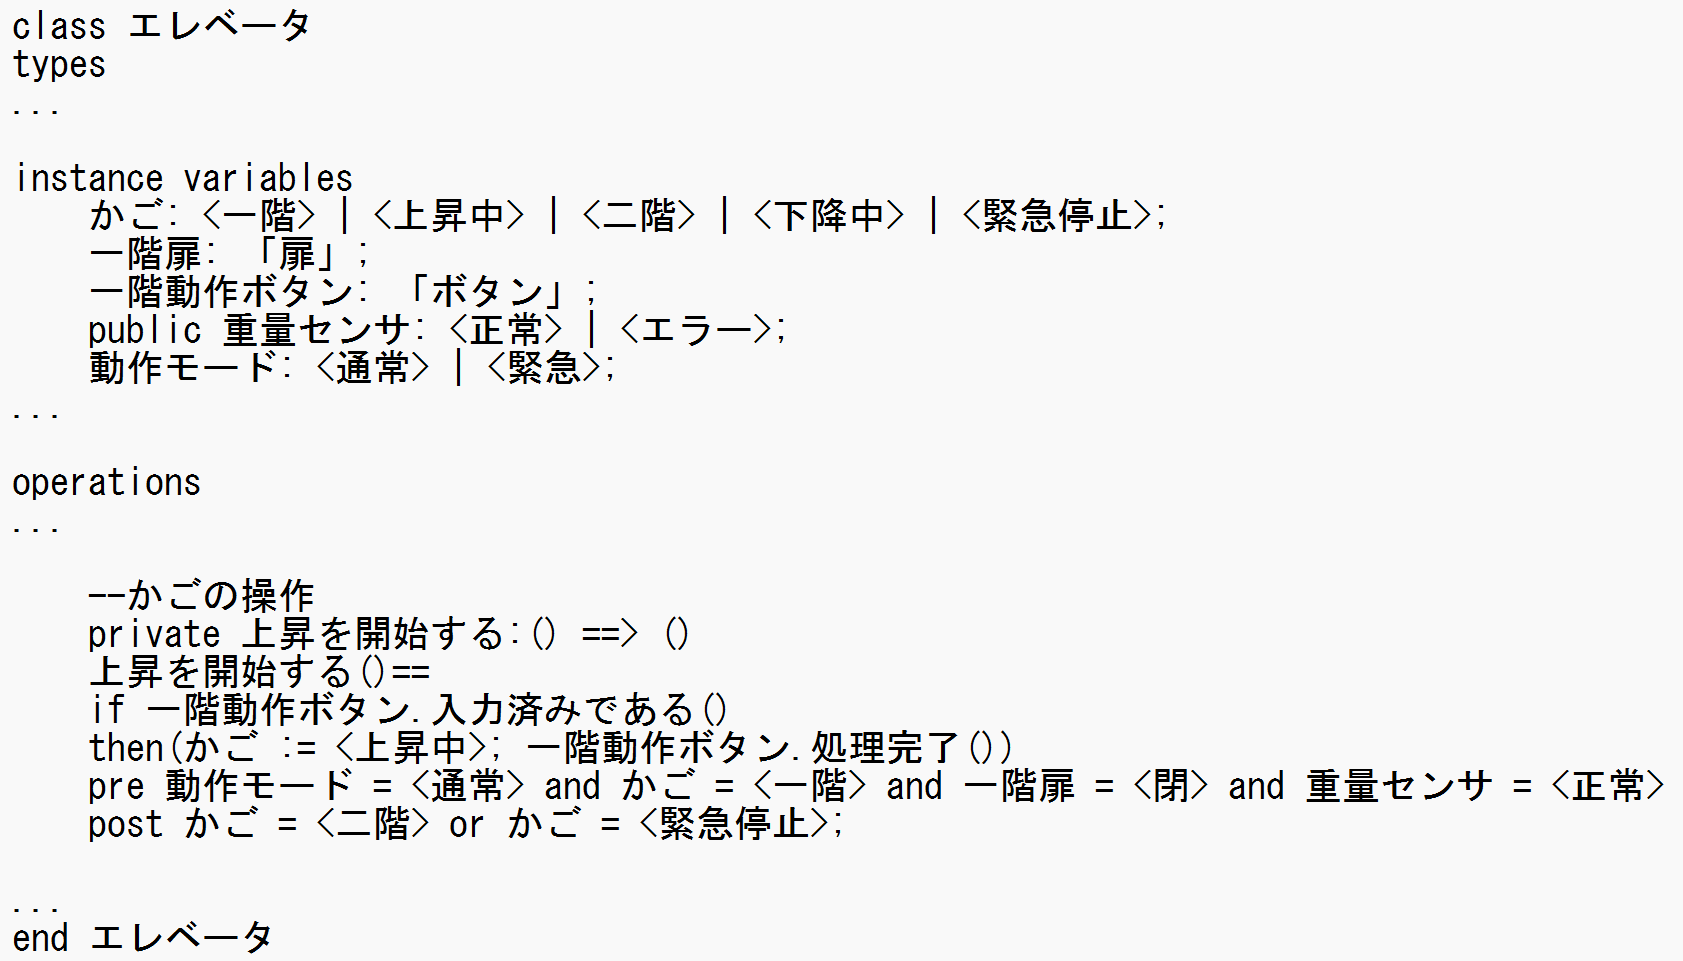
\includegraphics[width=\columnwidth]{../image/jceee/vdm_elevater.png}
      \caption{作成したVDM++仕様の一部}
      \label{fig:vdm_elevater}
\end{figure}

作成した自然言語仕様は、要求仕様13個で構成されており、VDM++仕様は、2つのクラスから構成され、定義が32個ある仕様である。

これらの仕様に対して、提案手法を適用した結果、自然言語仕様とVDM++仕様の対応関係を正しく抽出していることを確認した。
例えば、図\ref{fig:vdm_elevater}に示すクラス定義「エレベータ」に対して、
図\ref{fig:nat_elevater}に示す、名詞「エレベータ」を含むすべての要求仕様「elevator-110-11」、「elevator-110-12」、「elevator-110-13」、「elevator-110-14」
との対応関係を抽出していることを確認した。
また、図\ref{fig:vdm_elevater}中の「上昇を開始する」という操作定義に対して、
図\ref{fig:nat_elevater}に示す、「elevator-110-11」という要求仕様との対応関係を抽出していることを確認した。

\section{考察}
提案手法は、表\ref{tab:correspondence_rule}の規則にしたがって対応関係を抽出する。
これに対して、本論文では、表\ref{tab:correspondence_rule}の規則を満たす自然言語仕様とVDM++仕様の組に提案手法を適用し、
正しく対応関係を抽出することを確認できた。
これより、提案手法は自然言語仕様とVDM++仕様の対応関係を把握する際に有用であるといえる。
以上のことから、提案手法は自然言語仕様とVDM++仕様を併用し、仕様の変更や修正を行う際に発生する、
対応漏れの削減と、手間の削減に役立つといえる。

一方で、提案手法は現在、対応関係の抽出のみを行うため、抽出した対応関係をどのように活用するかは利用者に委ねられているという課題がある。
そこで、提案手法を用いて抽出した対応関係をもとに、
一方の仕様に変更があった際に、もう一方の仕様の影響範囲を明示的に提示する機能を持つツールを開発することで、
仕様変更時の影響範囲を把握しやすくし、対応漏れを防ぐことや、仕様の変更作業の手間と時間の削減に、さらに寄与できると考える。

\section{おわりに}
本論文では、自然言語仕様とVDM++仕様のトレーサビリティの維持を支援することを目的として、
両仕様の対応関係を自動で抽出する手法を提案した。
適用例として、表\ref{tab:correspondence_rule}の規則に従った自然言語仕様とVDM++仕様を用いて、
対応関係を正しく抽出できることを確認した。

以下に、本論文における今後の課題を示す。
\begin{itemize}
      \setlength{\itemsep}{-2pt}
      \item 構成子の対応関係の抽出
      \item 対応関係を抽出する規則の緩和
      \item 片方の仕様の変更に応じて、もう片方の仕様書の影響範囲を示す機能を持つツールの開発 % 機能の実装だと、もうツール化しているみたいでいやん
\end{itemize}

\begin{thebibliography}{99}
      \bibitem{spec_introduction}IPA独立行政法人 情報処理推進機構: 実務家のための形式手法\space
      厳密な仕様記述を志すための形式手法入門\space 厳密な仕様記述入門,
      \url{https://www.ipa.go.jp/archive/digital/iot-en-ci/keishikisyuho/hjuojm000000m6wx-att/000026829.pdf}. Accessed:2025.07.02

      \bibitem{successful_example}IPA独立行政法人 情報処理推進機構: 厳密な仕様記述における形式手法成功事例調査報告書,
      \url{https://www.ipa.go.jp/archive/digital/iot-en-ci/keishikisyuho/hjuojm000000m6wx-att/000026875.pdfL}. Accessed:2025.07.02

      \bibitem{vdm}International Organization for Standardization: ``ISO/IEC 13817-1:1996,
      Information technology — Programming languages, their environments and system software interfaces
      — Vienna Development Method — Specification Language - Part 1: Base language'', 1996.
\end{thebibliography}

\end{document}
